\documentclass[5p,twocolumn,10pt,times]{elsarticle}
\usepackage{amsmath}
\usepackage{hyperref}
\usepackage{booktabs}
\usepackage{listings}
\usepackage{multirow}
\usepackage{placeins}
\usepackage{tikz}
\usetikzlibrary{positioning}
\definecolor{primaryblue}{RGB}{31,78,121}

\newcommand{\cmark}{\ding{51}}% checkmark
\newcommand{\xmark}{\ding{55}}% x mark

%\modulolinenumbers[5]
\addtolength{\textheight}{8mm}
\addtolength{\textwidth}{4mm}
\addtolength{\voffset}{-10mm}
\addtolength{\hoffset}{-3mm}

\bibliographystyle{elsarticle-num}
\begin{document}
\baselineskip11pt

\begin{frontmatter}

\title{CADence: CAD Intelligence, A Multi-Agent Pipeline for Zero-Shot Text-to-CAD Generation with Parametric Expression Preservation}


% \author{First Author}
% \cortext[mycorresponingauthor]{Corresponding author}
% \ead{first@firstuni.edu}
% \author{Second Author}
% \address{Department of Mathematics, Stanford University}
% \author{Third Author}
% \address{Department of Computer Science, Tel Aviv University}

% \author{Important: the names of the authors, as well as other identity-revealing information (e.g. funding bodies), should be removed from the original submission to comply with the double-blind review process}


\begin{abstract} 
Generating parametric CAD models from natural language remains a significant challenge in geometric modeling. Existing approaches either require extensive fine-tuning on large annotated datasets or produce non-parametric code with hardcoded values. We present CADence, a multi-agent pipeline that generates parametric OpenSCAD models from text descriptions and images without any task-specific training. CADence introduces a JSON-based intermediate representation that preserves parametric expressions as strings throughout the generation process, enabling true design customization. The pipeline employs six coordinated stages: understanding, planning, compilation, rendering, visual self-correction, and component verification. Key innovations include a 6-view visual language model assessment system for comprehensive spatial evaluation, a 5-layer error recovery mechanism for robust generation, and tiered part validation with context-aware confidence thresholds. We evaluate CADence on a diverse set of over 150 prompts spanning three categories: mechanical components (gears, brackets, enclosures, motor mounts), everyday objects (mugs, chairs, lamps, storage containers), and abstract geometric designs (interlocking shapes, lattices, organic forms), demonstrating competitive results with fine-tuned approaches while offering superior parametric flexibility. On a curated benchmark of 15 prompts with ground truth dimensioned using parametric specifications from NopSCADlib~\cite{nopscadlib}, a widely-used open-source mechanical CAD library, CADence reduces Chamfer Distance relative to direct LLM generation on medium and complex designs. Across all evaluations, CADence achieves 100\% compilation and rendering success regardless of model configuration, owing to the multi-layer error recovery system. This eliminates the ``no output'' failure mode that limits direct generation approaches. Comprehensive ablation studies quantify the contribution of each architectural component: VLM self-correction raises approval rates from 0\% to 66.7\% over three iterations, component verification achieves an 86.4\% pass rate, and the hybrid model configuration attains 98.3\% parts detection. CADence represents a new paradigm for text-to-CAD generation that prioritizes inspectability, debuggability, and parametric design.
\end{abstract}

\begin{keyword} Text-to-CAD, Parametric modeling, Large language models, OpenSCAD, Multi-agent systems
\end{keyword}

\end{frontmatter}

%\linenumbers
%% ============================================================
\section{Introduction}
\label{sec:intro}
%% ============================================================
Computer-aided design (CAD) serves as the foundation for modern manufacturing, enabling engineers and designers to create precise geometric models that translate directly into physical products. Despite decades of advancement in CAD software, the barrier to entry remains high: users must master complex interfaces, understand geometric constraints, and possess domain expertise to translate design intent into valid models. Natural language offers an intuitive alternative, allowing users to describe what they want rather than how to construct it.

Recent advances in large language models (LLMs) have sparked interest in text-to-CAD generation, where natural language descriptions are automatically converted into executable CAD code. This capability could democratize design by enabling non-experts to create functional 3D models and accelerate the workflow of experienced designers. However, the problem presents unique challenges that distinguish it from other code generation tasks. CAD code must satisfy geometric constraints, produce renderable output, and ideally preserve parametric relationships that allow downstream customization. For instance, a cylindrical container defined by width \texttt{W}, height \texttt{H}, and wall thickness \texttt{t} should maintain expressions like \texttt{W/2 - t} for the inner radius, enabling users to adjust proportions without rewriting code. Losing these relationships by evaluating them to constants eliminates the primary benefit of parametric CAD.

Existing approaches to text-to-CAD generation fall into two categories. The first category involves fine-tuning language models on large datasets of text-CAD pairs. CAD-Coder~\cite{cadcoder2025} fine-tunes Qwen2.5-7B on 110,000 text-CadQuery pairs using supervised learning followed by reinforcement learning with geometric rewards. Text-to-CadQuery~\cite{text2cadquery2025} augments the Text2CAD dataset with 170,000 CadQuery annotations and trains multiple open-source models of varying sizes. Mind-CAD~\cite{mindcad2025} introduces a domain-specific language with a generator-planner-executor architecture, training on paired text-CAD data with depth and normal supervision. While these methods achieve strong results on their respective benchmarks, they require substantial training data and computational resources, and the resulting models may not generalize well to novel design categories. The second category leverages pre-trained LLMs in a zero-shot~\cite{li2025llm4cad} or few-shot manner~\cite{alrashedy2024generating}. These approaches avoid the cost of fine-tuning but face challenges with geometric reasoning and error recovery. Direct code generation without intermediate planning often produces syntactically valid but semantically incorrect models, and errors are difficult to diagnose and repair without structured representations.

Critically, both categories fail to preserve parametric relationships. Fine-tuned models typically output code with evaluated constants rather than symbolic expressions, while zero-shot methods lack the structured representations needed to maintain these relationships through generation. This limitation undermines the core proposition of parametric CAD: the ability to adjust designs without rewriting code.

We propose CADence, a multi-agent pipeline that addresses these limitations through three key innovations. First, we introduce a JSON-based intermediate representation (IR) that separates design planning from code generation. This separation enables inspection and modification of the design plan before compilation, makes errors easier to localize and repair, and crucially preserves parametric expressions as strings rather than evaluating them prematurely. Second, we develop a comprehensive visual feedback system that renders models from six orthographic views and employs visual language models (VLMs) to assess geometric accuracy. This multi-view approach captures spatial relationships that single-image assessment would miss. Third, we implement a 5-layer error recovery mechanism that progressively addresses issues from schema validation through manual repair hints, ensuring robust generation even for complex designs.

CADence targets OpenSCAD as its output format, a declarative language well-suited for parametric modeling. Unlike imperative CAD APIs, OpenSCAD's functional style aligns naturally with LLM generation, and its built-in customizer interface allows end users to adjust parameters without modifying code. Our pipeline preserves expressions like \texttt{W/2} and \texttt{H - wall\_t} throughout generation, producing truly parametric models that can be customized after creation. We evaluate CADence on a diverse set of over 150 prompts spanning three categories: mechanical components (gears, brackets, enclosures, motor mounts), everyday objects (mugs, chairs, lamps, storage containers), and abstract geometric designs (interlocking shapes, lattices, organic forms), demonstrating that zero-shot generation with structured planning can achieve competitive results with fine-tuned approaches while offering superior parametric flexibility. A curated benchmark with NopSCADlib-dimensioned ground truth confirms that CADence reduces Chamfer Distance relative to direct LLM generation on medium and complex designs. Across all evaluations, CADence achieves 100\% compilation and rendering success regardless of model configuration, eliminating the ``no output'' failure mode that limits direct generation approaches. Comprehensive ablation studies across multiple model configurations, VLM iteration counts, and verification strategies quantify the contribution of each pipeline stage, with VLM self-correction and component verification providing the largest gains. We release our implementation to support future research in this direction.

The remainder of this paper is organized as follows. Section~\ref{sec:related} reviews related work in text-to-CAD generation and LLM-based code synthesis. Section~\ref{sec:method} describes the CADence architecture in detail. Section~\ref{sec:experiments} presents our experimental setup, and Section~\ref{sec:results} reports quantitative and qualitative results. Section~\ref{sec:discussion} discusses limitations and future directions, and Section~\ref{sec:conclusion} concludes.

%% ============================================================
\section{Prior work}
\label{sec:related}
%% ============================================================

The integration of large language models with computer-aided design has emerged as a rapidly evolving research area. Zhang et al.~\cite{zhang2026llmcad} provide a comprehensive survey of this intersection, categorizing LLM applications in CAD into six key areas: data generation, CAD code generation, parametric CAD generation, image generation, model evaluation, and text generation. We focus on CAD code generation approaches, which can be divided into supervised fine-tuning methods that require large paired datasets and zero-shot methods that leverage pre-trained models. We then discuss relevant work on LLM-based code generation architectures, visual feedback systems, and parametric modeling techniques that inform our approach.

% Their analysis reveals that GPT-4o and GPT-4 are the most frequently employed models, and that nearly all current approaches generate intermediate representations rather than directly outputting 3D models. This observation validates the design philosophy underlying CADence, which introduces a structured JSON intermediate representation to bridge natural language understanding and geometric code generation.

\begin{table*}[t]
\centering
\caption{Comparison of CADence with concurrent text-to-CAD methods. CADence uniquely combines zero-shot operation with a JSON intermediate representation and multi-view VLM feedback, eliminating the need for large-scale training data while maintaining interpretability.}
\label{tab:method-comparison}
\begin{tabular}{lcccc}
\toprule
Aspect & CADence & CAD-Coder & Text-to-CadQuery & Mind-CAD \\
\midrule
Training Required & None (zero-shot) & 110K pairs + RL & 170K annotations & Dataset + supervision \\
Intermediate Representation & JSON IR & None (direct) & None (direct) & DSL \\
Target Language & OpenSCAD & CadQuery & CadQuery & Custom DSL \\
Feedback Mechanism & 6-view VLM & Geometric (CD) & None & Depth/Normal maps \\
Visual Input Support & Single + Multi-view & \xmark & \xmark & \xmark \\
Parametric Expressions & Full (string-preserved) & Limited & Limited & Limited \\
Error Recovery & 5-layer system & RL-based & None & None \\
KB/Component Library & NopSCADlib RAG & \xmark & \xmark & \xmark \\
\bottomrule
\end{tabular}
\end{table*}

% Early deep learning approaches for CAD generation focused on learning representations from existing designs. DeepCAD~\cite{wu2021deepcad} introduced a transformer-based autoencoder for CAD command sequences, demonstrating that neural networks could learn meaningful representations of geometric operations. Subsequent work extended this paradigm to conditional generation, where text or image inputs guide the decoding process.
\subsection{Supervised Fine-Tuning Approaches}

Recent supervised approaches to text-to-CAD generation fine-tune large language models on paired text-code datasets, building on earlier work in learned CAD representations~\cite{wu2021deepcad}, achieving strong performance through task-specific training. CAD-Coder~\cite{cadcoder2025} represents a significant advance in supervised text-to-CAD generation. The approach fine-tunes Qwen2.5-7B on a curated dataset of 110,000 text-CadQuery pairs, employing a two-stage training strategy. The first stage uses supervised fine-tuning (SFT) to learn the mapping from descriptions to code. The second stage applies Group Relative Policy Optimization (GRPO), a reinforcement learning algorithm that optimizes for geometric accuracy measured by Chamfer Distance between generated and ground-truth meshes. CAD-Coder also incorporates chain-of-thought reasoning to improve performance on complex designs. However, the reliance on geometric rewards requires access to ground-truth 3D models during training, limiting applicability to datasets with paired text-mesh annotations. Moreover, the direct code generation approach provides no mechanism for preserving parametric expressions, as the model outputs complete programs without intermediate structure.

Text-to-CadQuery~\cite{text2cadquery2025} takes a data-centric approach, arguing that scaling training data is more effective than architectural innovations. The authors augment the Text2CAD dataset with CadQuery annotations, yielding 170,000 training pairs. They fine-tune six open-source LLMs ranging from small to large parameter counts, demonstrating that model performance scales predictably with data and parameters. Their best model achieves 69.3\% exact match and 48.6\% Chamfer Distance reduction compared to baselines. While impressive, this approach inherits the limitations of direct code generation: outputs lack intermediate structure for debugging, and parametric relationships are typically lost to evaluated constants.

Mind-CAD~\cite{mindcad2025} introduces architectural innovations for the text-to-CAD problem. The system defines a domain-specific language (DSL) that abstracts common CAD operations, reducing the complexity of the generation target. A generator-planner-executor architecture decomposes the task into subtasks handled by specialized modules. The planner produces high-level operation sequences that the executor translates into concrete code. Mind-CAD also incorporates depth and normal map supervision during training, providing geometric feedback beyond discrete rewards. The EditBench dataset introduced alongside Mind-CAD enables the evaluation of iterative refinement capabilities. While the DSL provides structure, it constrains expressiveness to predefined operations and still requires substantial training data.

Our work differs from these approaches in several respects. Unlike CAD-Coder and Text-to-CadQuery, CADence operates in a zero-shot setting without task-specific training, making it immediately applicable to new domains. Unlike Mind-CAD, our intermediate representation preserves the full expressiveness of the target language (OpenSCAD) rather than constraining generation to a predefined DSL. The JSON IR enables inspection and modification of plans before compilation, a capability absent from direct code generation approaches. As noted by Zhang et al.~\cite{zhang2026llmcad}, evaluation inconsistency remains a challenge in this field; we address this by reporting multiple complementary metrics including geometric accuracy, semantic correctness, and parametric flexibility.

A further distinction concerns evaluation methodology. Prior supervised methods generate synthetic text prompts from existing CAD models using LLMs, creating a closed loop where the training and evaluation distributions are aligned by construction. CADence instead uses human-curated prompts drawn from real engineering documentation---specifically, the NopSCADlib component catalog---ensuring that evaluation reflects authentic design intent rather than artifacts of LLM paraphrasing.

\subsection{LLM-Based Code Generation}

Large language models have demonstrated remarkable code generation capabilities across programming languages. Codex~\cite{chen2021codex} showed that scaling GPT-3 and fine-tuning on code corpora produces models capable of solving programming challenges. Subsequent work has explored prompting strategies, tool use, and multi-agent architectures to improve reliability.

Multi-agent systems decompose complex tasks among specialized components that communicate through defined protocols. For code generation, this often involves separate agents for planning, implementation, testing, and debugging. Recent work demonstrates that such architectures outperform monolithic models on complex programming tasks by enabling iterative refinement and error correction.

Visual feedback has emerged as a powerful mechanism for code generation in domains with visual outputs. Systems that render generated code and use VLMs to assess results can identify semantic errors invisible to syntactic analysis. This approach is particularly valuable for graphics and visualization code, where correctness depends on visual appearance rather than test cases.

CADence combines insights from these directions. Our multi-agent architecture separates understanding, planning, compilation, and verification into distinct stages with well-defined interfaces. Visual feedback through 6-view rendering enables comprehensive geometric assessment, and our 5-layer error recovery provides robust handling of failures at each stage.

\subsection{Parametric CAD and Design Customization}

Parametric modeling represents geometric shapes through parameters and constraints rather than explicit coordinates. This representation enables design exploration by varying parameters and supports downstream applications like optimization and manufacturing planning. Traditional CAD systems have long supported parametric modeling, but automated generation of parametric designs remains challenging.

Most text-to-CAD systems produce code with hardcoded values, losing the parametric relationships implicit in the input description. A user who requests a ``cylindrical container with wall thickness proportional to diameter'' expects the output to maintain this relationship when parameters change. Achieving this requires preserving expressions throughout generation rather than evaluating them prematurely.

OpenSCAD provides a natural target for parametric generation due to its declarative semantics. Parameters defined at the top of a script propagate through all expressions that reference them, and the built-in customizer interface exposes parameters for interactive adjustment. CADence exploits these features by preserving expressions as strings in its JSON IR and generating OpenSCAD code that maintains parametric relationships.


%% ============================================================
\section{Method}
\label{sec:method}
%% ============================================================
CADence is a multi-agent pipeline that transforms natural language descriptions and optional images into parametric OpenSCAD code. The pipeline consists of six stages, each implemented as an independent agent with defined inputs and outputs. Figure~\ref{fig:pipeline} illustrates the overall architecture.

\subsection{Pipeline Overview}

The pipeline processes inputs through the following stages:

\textbf{Stage 1: Understanding.} The VisionAnalyzer processes any input images, extracting geometric features, dimensions, and spatial relationships. For multi-view inputs, it synthesizes information across views to form a coherent 3D understanding. The TextReasoner analyzes the text prompt to identify required components, classify them into essential, secondary, and optional tiers, and extract dimensional parameters. A knowledge base detector identifies references to standard components (e.g., NEMA motors, common fasteners) that can be retrieved from the NopSCADlib library.

\textbf{Stage 2: Planning.} The Planner generates a JSON CAD plan that specifies geometry, operations, and parameters. This intermediate representation preserves parametric expressions as strings, enabling downstream stages to generate code with intact relationships. The plan undergoes schema validation to ensure structural correctness before proceeding.

\textbf{Stage 3: Compilation.} The Compiler translates the JSON plan into OpenSCAD code, maintaining expression strings and generating appropriate parameter ranges for the customizer interface. The output includes modular function definitions and a clear assembly structure.

\textbf{Stage 4: Rendering.} The OpenScadRunner invokes OpenSCAD to render the generated code from six orthographic viewpoints: front, back, left, right, top, and bottom. These views provide comprehensive spatial coverage for visual assessment. Timeout handling detects computationally expensive operations like hull and minkowski applied to complex bodies.

\textbf{Stage 5: VLM Self-Correction.} The VisualSelfCorrector presents the six rendered views to a visual language model along with the original prompt. The VLM assesses whether the model matches the description, identifies specific issues, and suggests corrections. If the assessment indicates problems, the system generates targeted fixes and iterates.

\textbf{Stage 6: Component Verification.} The ComponentVerifier checks that all expected parts are present and properly connected using tiered confidence thresholds. Essential parts require 85\% confidence, secondary parts require 65\%, and optional parts require 50\%. This reflects the intuition that a car without wheels fails validation, but a car without door handles may still be acceptable.

\begin{figure*}[!t]
\centering
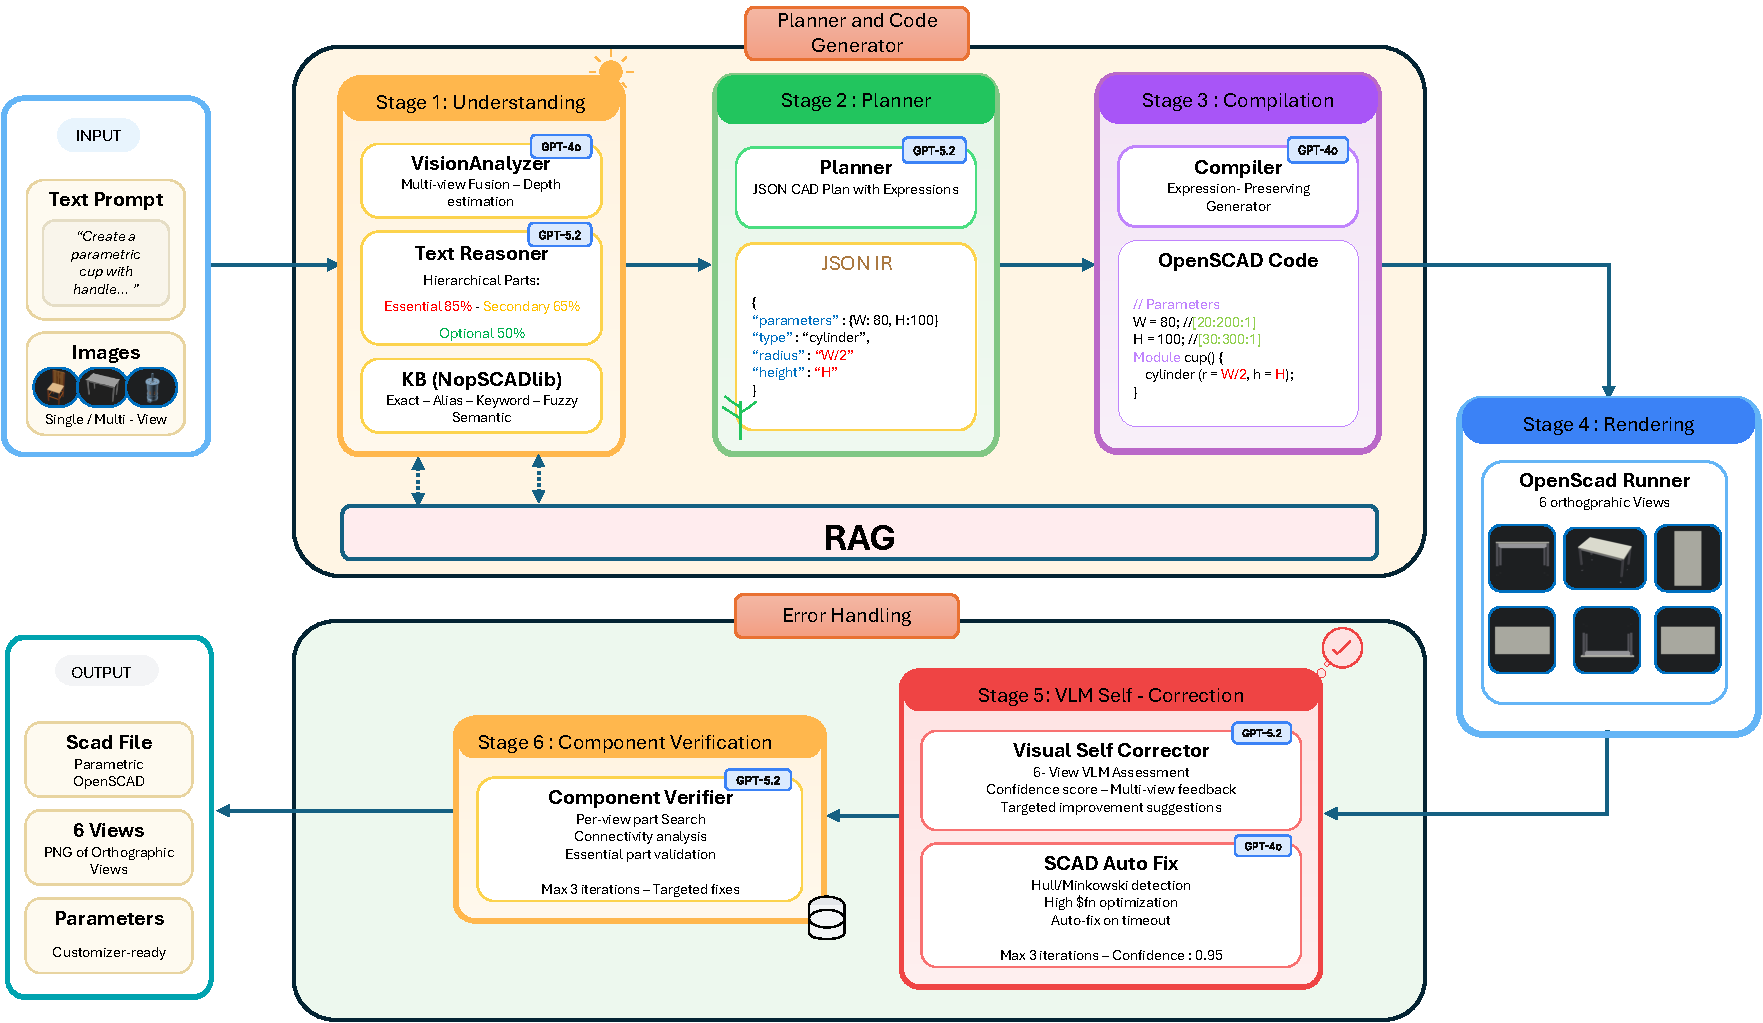
\includegraphics[width=\textwidth]{figures/pdf/CAD_Pipeline.pdf}
\caption{CADence pipeline architecture comprising two subsystems: \textbf{Planner and Code Generator} (Stages 1--3) transforms text/image inputs into parametric OpenSCAD via JSON intermediate representation with preserved expressions; \textbf{Error Handling} (Stages 5--6) ensures quality through 6-view VLM assessment and tiered component verification (Essential 85\%, Secondary 65\%, Optional 50\%). Stage 4 renders orthographic views connecting both subsystems. RAG-based NopSCADlib integration enables standard component reuse.}
\label{fig:pipeline}
\end{figure*}

\subsection{JSON Intermediate Representation}

A central innovation of CADence is the JSON-based intermediate representation that mediates between understanding and code generation. The schema defines three required sections: metadata, parameters, and geometry.

The metadata section specifies version information, units, and a human-readable description. The parameters section defines named parameters with optional range constraints for the customizer. Crucially, parameter values can be numbers or expressions referencing other parameters.

The geometry section contains base shapes and operations. Base shapes include primitives (box, cylinder, sphere, cone, torus) and extrusions (linear\_extrude, rotate\_extrude). Each shape has an identifier, type-specific dimensions, position, and rotation. Dimensions can be numbers or string expressions like \texttt{"W/2"} or \texttt{"H - wall\_t"}.

Operations transform and combine shapes through CSG operations (union, difference, intersection), spatial transformations (translate, rotate, scale, mirror), and advanced operations (hull, minkowski). Each operation specifies its type, target shapes, and any additional parameters.

This representation offers several advantages over direct code generation. Plans can be inspected and modified before compilation, making errors easier to localize. Schema validation catches structural problems early, before code generation. The separation of planning and compilation allows alternative backends (e.g., CadQuery, FreeCAD) without changing the planning stage. Most importantly, preserving expressions as strings ensures that parametric relationships survive to the final output.

\subsection{Parametric Expression Preservation}

Unlike prior approaches that evaluate expressions during generation, CADence preserves parametric relationships throughout the pipeline. Consider a cylindrical container defined by width $W$, height $H$, and wall thickness $t$. The JSON plan represents the outer cylinder with radius \texttt{"W/2"} and the inner cylinder with radius \texttt{"W/2 - wall\_t"}. These strings flow unchanged through compilation to produce OpenSCAD code:

\begin{lstlisting}[language=C,caption={Parametric OpenSCAD output}]
W = 100; //[20:300:1]
H = 50;  //[10:150:1]
wall_t = 2; //[1:10:0.5]

module outer_cylinder() {
  cylinder(h=H, r=W/2, center=true);
}
module inner_cylinder() {
  cylinder(h=H+1, r=W/2-wall_t, center=true);
}
\end{lstlisting}

The compiler automatically generates parameter ranges based on semantic analysis. Width, height, and length parameters receive ranges from 20\% to 300\% of their default values. Thickness parameters receive ranges from 50\% to 500\%. Angles range from 0 to 360 degrees. These heuristics produce reasonable customization bounds without manual specification.

\begin{figure*}[t]
\centering
\includegraphics[width=\linewidth]{figures/pdf/Parametric_table_CAD_model.pdf}
\caption{Parametric customization of a CADence-generated table. The original model (center, top rows) can be modified through parameter adjustments: changing table top color (red variants, bottom left) or leg color (blue variant, bottom right) while preserving geometric relationships. This demonstrates how preserved parametric expressions enable downstream design exploration without regenerating the model.}
\label{fig:parametric}
\end{figure*}

\subsection{6-View VLM Assessment}
\label{subsec:vlm}

Single-image assessment can miss geometric issues visible only from specific angles. A model that appears correct from the front may have incorrect depth or missing features visible from the side. CADence addresses this by rendering six orthographic views and presenting them together for VLM assessment.

The views are configured with cameras at fixed distances along each axis, with appropriate up vectors for consistent orientation. The VLM receives all six images along with the original prompt and responds with a structured assessment including approval status, confidence score, identified issues, suggested fixes, and per-view feedback.

The assessment prompt instructs the VLM to check for blank images (indicating render failures), match between the model and description, geometric accuracy, completeness of specified features, and overall quality. The VLM operates with a reasoning model (GPT-5.2 in our implementation) to enable detailed spatial analysis.

If the assessment identifies issues with confidence below 0.95, the system generates targeted corrections and re-renders. This loop continues for up to three iterations, providing multiple opportunities to resolve problems while avoiding infinite cycles.

\subsection{5-Layer Error Recovery}
\label{subsec:recovery}

A persistent practical challenge in text-to-CAD generation is output fragility: systems frequently produce code that fails to compile, renders incorrectly, or omits critical components---yet offer no mechanism to recover from these failures. Among the concurrent methods surveyed in Table~\ref{tab:method-comparison}, CAD-Coder employs RL-based geometric rewards during training but provides no runtime error handling once a model is deployed; Text-to-CadQuery and Mind-CAD include no recovery mechanism at all. In practice, this means a substantial fraction of generation attempts yield no usable output---a critical limitation for any interactive design tool where users expect reliable results.

CADence addresses this gap through a 5-layer error recovery architecture (Figure~\ref{fig:recovery}) that provides progressive, bounded recovery from failures at each pipeline stage. The design follows two principles. First, layers are ordered by increasing computational cost: inexpensive deterministic fixes precede LLM-based corrections, which in turn precede human-in-the-loop intervention. This ordering minimizes API cost and latency for the common case where failures are structural rather than semantic. Second, each layer targets a distinct failure category---from malformed JSON schemas to subtle geometric omissions that only a visual language model or a human observer would catch---ensuring comprehensive coverage of the failure space.

\begin{figure*}[t]
\centering
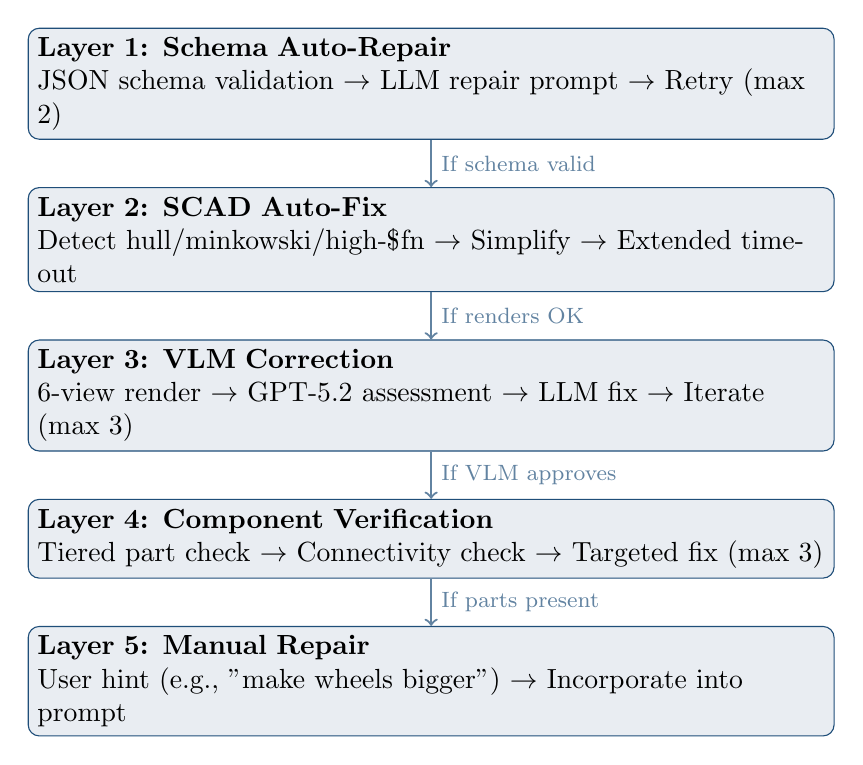
\begin{tikzpicture}[
    node distance=0.6cm,
    layer/.style={rectangle, draw=primaryblue, fill=primaryblue!10, text width=10cm, minimum height=1cm, align=left, rounded corners},
    arrow/.style={->, thick, primaryblue!70}
]

\node[layer] (l1) {\textbf{Layer 1: Schema Auto-Repair}\\JSON schema validation $\rightarrow$ LLM repair prompt $\rightarrow$ Retry (max 2)};
\node[layer, below=of l1] (l2) {\textbf{Layer 2: SCAD Auto-Fix}\\Detect hull/minkowski/high-\$fn $\rightarrow$ Simplify $\rightarrow$ Extended timeout};
\node[layer, below=of l2] (l3) {\textbf{Layer 3: VLM Correction}\\6-view render $\rightarrow$ GPT-5.2 assessment $\rightarrow$ LLM fix $\rightarrow$ Iterate (max 3)};
\node[layer, below=of l3] (l4) {\textbf{Layer 4: Component Verification}\\Tiered part check $\rightarrow$ Connectivity check $\rightarrow$ Targeted fix (max 3)};
\node[layer, below=of l4] (l5) {\textbf{Layer 5: Manual Repair}\\User hint (e.g., "make wheels bigger") $\rightarrow$ Incorporate into prompt};

\draw[arrow] (l1) -- node[right, font=\footnotesize] {If schema valid} (l2);
\draw[arrow] (l2) -- node[right, font=\footnotesize] {If renders OK} (l3);
\draw[arrow] (l3) -- node[right, font=\footnotesize] {If VLM approves} (l4);
\draw[arrow] (l4) -- node[right, font=\footnotesize] {If parts present} (l5);

\end{tikzpicture}
\caption{5-Layer Error Recovery Architecture. Each layer targets a distinct failure category, ordered by increasing computational cost. Layers 1--4 operate automatically with bounded retry budgets (max 10 total iterations); Layer~5 accepts optional user hints for cases requiring human judgment. This progressive design ensures that simple structural failures are resolved cheaply while complex semantic issues receive proportional attention.}
\end{figure*}


\textbf{Layer 1: Schema Auto-Repair.} The JSON plan produced by the Planner undergoes validation against a predefined schema that enforces required fields, type constraints, and structural invariants. When validation fails---common causes include missing geometry entries, malformed expression strings, or unsupported operation types---the error message and the offending plan are sent to the LLM with a targeted repair prompt. The LLM receives the schema definition alongside the specific validation errors, enabling focused correction rather than full regeneration. Up to two repair attempts are permitted before the pipeline proceeds with whatever valid structure has been recovered. This layer catches the majority of structural failures at negligible cost, since schema validation is deterministic and repair prompts are short.

\textbf{Layer 2: SCAD Auto-Fix.} Syntactically valid OpenSCAD code can still fail at render time due to computationally expensive operations. The auto-fixer analyzes generated code for known problematic patterns: \texttt{hull()} and \texttt{minkowski()} applied to bodies with many faces cause exponential rendering times, while high \texttt{\$fn} values (face counts exceeding 128) can produce multi-minute renders for operations that should complete in seconds. When these patterns are detected, the system applies targeted simplifications---replacing \texttt{hull()} with bounding-box approximations, capping \texttt{\$fn} at reasonable values---and retries with an extended timeout (120s vs.\ the default 60s). This layer operates deterministically without LLM calls, making it both fast and reliable.

\textbf{Layer 3: VLM Correction.} If the rendered model does not match the input description, the 6-view VLM assessment (Section~\ref{subsec:vlm}) provides structured feedback: a confidence score, specific identified issues (e.g., ``handle is attached to the wrong side''), and suggested corrections. These are incorporated into a correction prompt that targets the specific failing components rather than regenerating the entire design. The correction employs a reasoning model (GPT-5.2) to handle the spatial reasoning required for geometric fixes. Up to three iterations are permitted, with early stopping if the VLM confidence exceeds 0.95. This layer addresses semantic errors---models that compile and render but do not match the user's intent---which are invisible to purely syntactic checks.

\textbf{Layer 4: Component Verification.} The ComponentVerifier cross-references the rendered output against the expected parts list from Stage~1, applying tiered confidence thresholds (Essential 85\%, Secondary 65\%, Optional 50\%). When parts are missing or disconnected---detected through both visual analysis and connectivity checking---the system generates targeted fixes that address specific components without disturbing correct portions of the model. This targeted approach preserves work done in previous layers and avoids the regression risk of full regeneration. Up to three verification-repair iterations are allowed.

\textbf{Layer 5: Manual Repair.} When automatic recovery cannot resolve an issue---typically for subjective aesthetic concerns or ambiguous prompt interpretations---users can supply natural language hints such as ``make the wheels bigger'' or ``add a handle on the right side.'' The RepairOrchestrator incorporates these hints into a repair prompt alongside the current code and the original design brief, enabling human-guided refinement without requiring users to write OpenSCAD code directly. This layer bridges the gap between fully automated generation and manual CAD authoring, providing a graceful degradation path that ensures the system always produces a usable starting point for further refinement.

The total automatic iteration budget is bounded at 10 attempts (2 + 2 + 3 + 3 across Layers 1--4), providing substantial opportunity for recovery without unbounded computation or runaway API costs. This progressive architecture is, to our knowledge, unique among text-to-CAD systems: it transforms generation from a single-shot process with binary success/failure into a robust pipeline where each layer incrementally improves output quality. The practical consequence, as shown in Table~\ref{tab:model-config}, is that CADence achieves 100\% compilation success across all model configurations, even on complex multi-part assemblies---eliminating the ``no output'' failure mode that plagues direct generation approaches. Furthermore, the layered design means that the majority of recoveries are resolved in the inexpensive early layers (schema repair and auto-fix), with the costlier VLM-based layers engaged only when semantic issues persist.


\subsection{Knowledge Base Integration}

Many designs incorporate standard components like motors, sensors, and fasteners. Generating these from scratch is wasteful when high-quality implementations exist. CADence integrates with NopSCADlib, a comprehensive library of OpenSCAD modules for mechanical components.

The knowledge base detector employs five strategies with decreasing confidence: exact name matching (confidence 1.0), alias matching using predefined mappings (0.9), category keyword search (0.7), fuzzy string matching with Levenshtein distance (0.5--0.8), and semantic similarity via embedding search (variable). When components are detected, their specifications are retrieved and incorporated into the design brief.

The integration uses graceful fallback: if KB detection fails or no components are found, the pipeline continues with pure LLM generation. This ensures that KB unavailability never blocks generation, which is critical for production deployment.

\subsection{Model Allocation Strategy}

CADence employs a hybrid model strategy that balances capability against cost and latency. Components requiring complex reasoning use GPT-5.2, a reasoning-optimized model, while components performing more deterministic tasks use GPT-4o for faster response times. Table~\ref{tab:model-allocation} details the allocation and rationale for each pipeline component.

\begin{table*}[t]
\centering
\caption{Model allocation across pipeline stages. GPT-5.2 handles reasoning-intensive tasks requiring design understanding and visual assessment, while GPT-4o handles deterministic generation tasks where consistency and speed are prioritized.}
\label{tab:model-allocation}
\small
\begin{tabular}{lll}
\toprule
\textbf{Component} & \textbf{Model} & \textbf{Rationale} \\
\midrule
PromptEnhancer & GPT-4o & KB-augmented prompt refinement \\
TextReasoner & GPT-5.2 & Complex reasoning for design understanding \\
Planner & GPT-5.2 & Logical planning for JSON structure \\
VisionAnalyzer & GPT-4o & Fast, deterministic image analysis \\
SingleImageAnalyzer & GPT-5.2 & Advanced 3D inference from 2D \\
Compiler & GPT-4o & Deterministic code generation \\
RepairOrchestrator & GPT-4o & Deterministic repair tasks \\
VisualSelfCorrector & GPT-5.2 & Visual reasoning with 6 views \\
ComponentVerifier & GPT-5.2 & Detailed part assessment \\
\bottomrule
\end{tabular}
\end{table*}

This allocation reflects the observation that planning and assessment benefit from deliberative reasoning, while compilation and repair involve more mechanical transformations where speed matters more than depth. The modular design allows each component to be independently configured, enabling straightforward model substitution as newer models become available.



%% ============================================================
\section{Experiments}
\label{sec:experiments}
%% ============================================================

\subsection{Evaluation Protocol}

We evaluate CADence through two complementary protocols designed to assess both pipeline robustness and geometric accuracy.

\textbf{Pipeline evaluation (150+ prompts).} We evaluate CADence on a diverse set of over 150 prompts spanning three categories: mechanical components (gears, brackets, enclosures, motor mounts), everyday objects (mugs, chairs, lamps, storage containers), and abstract geometric designs (interlocking shapes, lattices, organic forms). Prompts are distributed across three complexity levels---simple (single-primitive shapes), medium (functional objects with multiple features), and complex (multi-part assemblies requiring domain knowledge). This evaluation set exercises all pipeline stages across multiple model configurations, VLM iteration counts, and component verification strategies, providing comprehensive coverage of the design space.

\textbf{Geometric benchmark (15 prompts).} For rigorous geometric comparison against baselines, we curate a benchmark of 15 prompts (5 per complexity level) targeting mechanical components whose parametric specifications are documented in NopSCADlib~\cite{nopscadlib}---a comprehensive, community-maintained open-source library of parametric OpenSCAD modules. Ground truth models are authored using the exact dimensions, mounting patterns, and tolerances specified in the NopSCADlib catalog (e.g., 608 bearing: 22mm OD, 8mm bore, 7mm width; NEMA~17: 42.3mm face, 31mm mounting pattern). This grounds the reference geometries in established, independently verifiable engineering specifications. \textit{Simple} prompts describe basic mechanical components (608 ball bearing, M8 flat washer, GT2 20-tooth pulley, 40mm fan mount plate, LM8UU linear bearing holder). \textit{Medium} prompts specify multi-feature designs requiring precise dimensions (NEMA~17 motor mount, MGN12 carriage mount, 608 bearing housing, SG90 servo bracket, Arduino Nano holder). \textit{Complex} prompts target multi-part assemblies requiring domain knowledge (GT2 belt tensioner with 608 idler, 5mm-to-8mm shaft coupler, Raspberry Pi~4 case, ESP32 enclosure with OLED, T8 leadscrew nut block).

For quantitative evaluation, we employ the following metrics. \textit{Compilation rate} measures the percentage of prompts that produce syntactically valid OpenSCAD code. \textit{Render success} measures the percentage that render within the timeout without errors. \textit{Validation score} measures geometric and semantic accuracy on a 0--100 scale. \textit{Parts detection} measures the percentage of expected components identified in final renders. \textit{VLM approval} measures the percentage approved by the visual assessment with confidence at least 0.85. For geometric accuracy, we compute Chamfer Distance (CD) between point clouds extracted from generated and reference meshes; lower CD indicates closer geometric match.

\subsection{Ablation Studies}

To understand the contribution of each component, we conduct ablation studies across our evaluation set, spanning simple, medium, and complex designs:

\textbf{Model Configuration.} We compare three model allocations---all GPT-4o, all GPT-5.2, and the CADence hybrid (GPT-4o for pipeline, GPT-5.2 for VLM/verification)---to quantify the trade-off between reasoning depth and generation speed.

\textbf{VLM Iteration Count.} We vary the number of VLM self-correction iterations from 0 to 3 to measure the marginal benefit of each additional feedback round.

\textbf{Component Verification.} We compare pipeline output before and after component verification with tiered confidence thresholds to isolate the contribution of the verification stage.

\subsection{Comparison with Prior Work}

Direct comparison with fine-tuned approaches is complicated by different output formats (OpenSCAD vs.\ CadQuery) and evaluation metrics. We therefore compare CADence against direct LLM generation baselines (GPT-4o and GPT-5.2 producing OpenSCAD in a single prompt) across our 15-prompt geometric benchmark with NopSCADlib-dimensioned ground truth. This isolates the benefit of the multi-stage pipeline architecture, JSON intermediate representation, and error recovery system over raw LLM capability. We additionally compare CADence with and without NopSCADlib RAG integration to quantify the contribution of knowledge base retrieval. While output format differences preclude exact metric-level comparison with CAD-Coder~\cite{cadcoder2025} and Text-to-CadQuery~\cite{text2cadquery2025}, we note that CADence operates entirely zero-shot---without any of the 110K+ training pairs these methods require---while producing fully parametric, customizable output. Although our evaluation uses 150 human-curated prompts compared to the 660K LLM-generated prompts employed by supervised methods, our focus is on engineering accuracy and zero-shot generalization rather than data-scale training. Each of our prompts is carefully authored to reflect realistic design tasks, providing a more meaningful signal of practical utility than large-scale synthetic benchmarks where prompt quality is variable.

\subsection{Implementation Details}

CADence is implemented in Python with approximately 12,000 lines across core pipeline, knowledge base, and utility modules. The system uses Flask for its web API and integrates with OpenSCAD for rendering. LLM calls use the OpenAI API with appropriate model selection per component.

Key configuration parameters include VLM confidence threshold (0.95), maximum VLM iterations (3), maximum component iterations (3), essential/secondary/optional part thresholds (0.85/0.65/0.50), initial render timeout (60s), and extended timeout for complex operations (120s).

All experiments use default configurations without per-prompt tuning. Temperature is set to 0 for deterministic components and 0.7 for creative planning.



%% ============================================================
\section{Results}
\label{sec:results}
%% ============================================================
\subsection{Overall Performance}

Across all evaluations, CADence achieves 100\% compilation and rendering success regardless of model configuration, owing to the multi-layer error recovery system (Section~\ref{subsec:recovery}). This eliminates the ``no output'' failure mode that limits direct generation approaches.

Table~\ref{tab:model-config} summarizes pipeline performance under three model configurations across the evaluation set. The hybrid configuration (GPT-4o for pipeline stages, GPT-5.2 for VLM and verification) achieves the highest parts detection rate (98.3\%) with a validation score of 89.8, while the all-GPT-5.2 configuration attains the highest validation score (95.2). Table~\ref{tab:complexity-comparison} reports Chamfer Distance on the 15-prompt geometric benchmark against NopSCADlib-dimensioned reference models. The structured pipeline consistently outperforms direct LLM generation, with the benefit increasing at higher complexity levels, demonstrating that the pipeline's advantage grows precisely where it is most needed.

\subsection{Ablation Results}
\textbf{Model Configuration.} Table~\ref{tab:model-config} compares three model configurations spanning simple, medium, and complex designs across the evaluation set. The all-GPT-5.2 configuration achieves the highest validation score (95.2), confirming the benefit of reasoning models for geometric understanding. However, the CADence hybrid configuration achieves the highest parts detection rate (98.3\%), suggesting that the combination of GPT-4o's consistent code generation with GPT-5.2's thorough visual assessment catches component omissions that either model alone would miss. The latency difference reflects this thoroughness: the hybrid configuration's VLM correction stage identifies more opportunities for refinement, leading to additional iterations. For applications prioritizing output completeness over generation speed, this represents a favorable tradeoff.

\begin{table}[t]
\centering
\caption{Model configuration comparison across the evaluation set. Validation score measures geometric and semantic accuracy (0--100). Parts detection measures percentage of expected components identified in final renders. All configurations achieve 100\% compilation and render success due to the multi-layer error recovery system.}
\label{tab:model-config}
\small
\begin{tabular}{lccc}
\toprule
\textbf{Configuration} & \textbf{Val. Score} & \textbf{Parts Det.} & \textbf{Latency} \\
\midrule
All GPT-4o & 80.9 & 85.9\% & 85.4s \\
All GPT-5.2 & \textbf{95.2} & 92.4\% & 154.3s \\
CADence (Hybrid) & 89.8 & \textbf{98.3\%} & 183.4s \\
\bottomrule
\end{tabular}
\end{table}
\textbf{VLM Iteration Count.} Table~\ref{tab:vlm-ablation} shows the effect of varying VLM self-correction iterations. Without VLM feedback (0 iterations), no prompts receive VLM approval. Each additional iteration improves the approval rate: 1 iteration yields 43.3\%, 2 iterations 60.0\%, and 3 iterations 66.7\%. The diminishing returns between iterations 2 and 3 suggest that three iterations provide a reasonable trade-off between quality improvement and computational cost. Average generation time increases from 65.0s without VLM to 142.2s with three iterations, confirming that the VLM correction loop is the primary cost driver.

\begin{table}[t]
\centering
\caption{Effect of VLM self-correction iterations across the evaluation set. Each additional iteration improves approval rate with diminishing returns. All configurations achieve 100\% compilation rate.}
\label{tab:vlm-ablation}
\small
\begin{tabular}{lccc}
\toprule
\textbf{Iterations} & \textbf{VLM Approval} & \textbf{Avg.\ Conf.} & \textbf{Avg.\ Time (s)} \\
\midrule
0 & 0.0\% & --- & 65.0 \\
1 & 43.3\% & 0.54 & 282.7 \\
2 & 60.0\% & 0.62 & 147.9 \\
3 & 66.7\% & 0.60 & 142.2 \\
\bottomrule
\end{tabular}
\end{table}

\textbf{Component Verification.} Table~\ref{tab:verif-ablation} shows the impact of the tiered component verification stage. Before verification, expected parts are not formally validated against the design brief. After verification with tiered thresholds (Essential 85\%, Secondary 65\%, Optional 50\%), 90.9\% of essential parts and 83.3\% of secondary parts are correctly detected, yielding an overall verification pass rate of 86.4\%. The lower detection rate for optional parts (28.6\%) reflects the design intent: optional features such as decorative elements are frequently absent from generated models without compromising functional correctness.

\begin{table}[t]
\centering
\caption{Impact of component verification with tiered confidence thresholds across the evaluation set. Essential parts are detected at the highest rate, reflecting the tiered threshold design.}
\label{tab:verif-ablation}
\small
\begin{tabular}{lcccc}
\toprule
\textbf{Stage} & \textbf{Essential} & \textbf{Secondary} & \textbf{Optional} & \textbf{Pass Rate} \\
\midrule
Before & 0.0\% & 0.0\% & 0.0\% & 0.0\% \\
After & 90.9\% & 83.3\% & 28.6\% & 86.4\% \\
\bottomrule
\end{tabular}
\end{table}

\textbf{Pipeline vs.\ Direct Generation.} The benefit of the JSON intermediate representation and multi-stage pipeline can be inferred from the Chamfer Distance comparison in Table~\ref{tab:complexity-comparison}. On medium-complexity prompts, the best CADence configuration achieves a CD of 5.91 compared to 8.65 for direct GPT-5.2 generation---a 32\% reduction attributable to structured planning, error recovery, and knowledge base retrieval. On complex prompts, CADence achieves 10.54 vs.\ 14.76 for GPT-5.2 (29\% reduction), demonstrating that the pipeline's advantage grows with design complexity.

\textbf{KB Integration.} Internally, comparing CADence with and without RAG reveals that knowledge base retrieval provides the largest benefit on medium-complexity designs (CD 5.91 vs.\ 7.51, a 21\% improvement), where standard component specifications---such as bearing dimensions and mounting hole patterns---are most informative. For complex designs, the pipeline's iterative VLM correction contributes more than RAG, as these designs require spatial reasoning beyond what can be retrieved from component datasheets.

\subsection{Comparison Results}
%% ============================================================
%% FIGURE 1: Main Comparison Figure (Full-width)
%% Place in Section 5 (Results) - Comparison Results subsection
%% ============================================================

\begin{figure*}[t]
\centering
\includegraphics[width=\textwidth]{figures/png/qualitative_comparison.png}
\caption{Qualitative comparison across prompt complexity levels. Direct LLM generation (GPT-4o, GPT-5.2) succeeds on simple primitives but degrades on functional objects and fails on complex assemblies requiring domain knowledge. CADence maintains quality across all levels through its JSON intermediate representation and multi-view VLM feedback. CADence + RAG further improves on mechanical components by retrieving accurate specifications from NopSCADlib (e.g., correct NEMA17 mounting hole patterns, standard bearing dimensions).}
\label{fig:comparison}
\end{figure*}

\begin{figure*}[t]
\centering
\caption{Multi-view rendering outputs from CADence. Each row shows a generated model from text prompt: the main isometric output (left) followed by the six orthographic views used for VLM assessment. This comprehensive spatial coverage enables detection of geometric issues invisible from any single viewpoint—note how internal features (mounting holes, cavities) are only visible from specific orientations.}
\label{fig:multiview}
\vspace{2mm}

\setlength{\tabcolsep}{2pt}
\renewcommand{\arraystretch}{1.2}
\small

\begin{tabular}{p{2.8cm}|c|cccccc}
\toprule
\textbf{Prompt} & \textbf{Output} & \textbf{Front} & \textbf{Back} & \textbf{Left} & \textbf{Right} & \textbf{Top} & \textbf{Bottom} \\
\midrule

% Row 1: NEMA17 + Fan (complex assembly)
\raggedright Cooling fan on NEMA17 motor with 10mm standoff bracket &
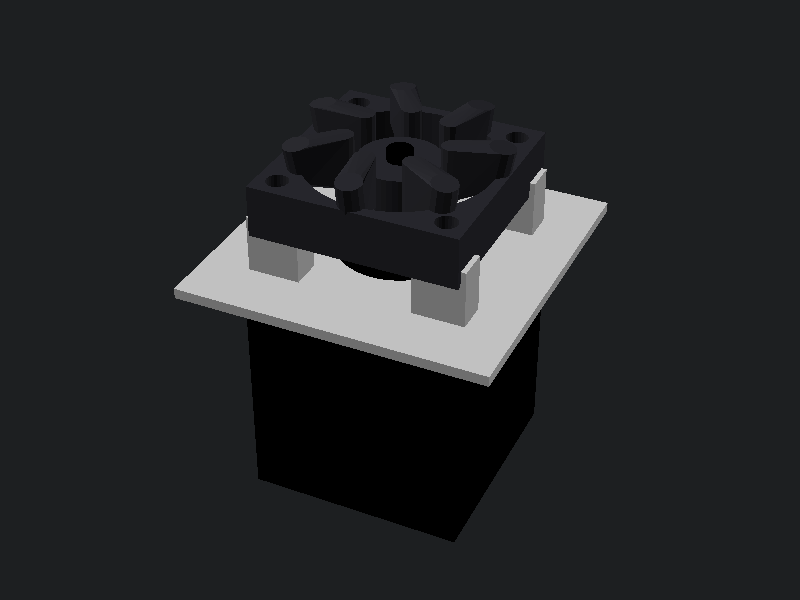
\includegraphics[width=1.9cm,height=1.9cm,keepaspectratio]{figures/png/nema_fan/nema_fan_iso.png} &
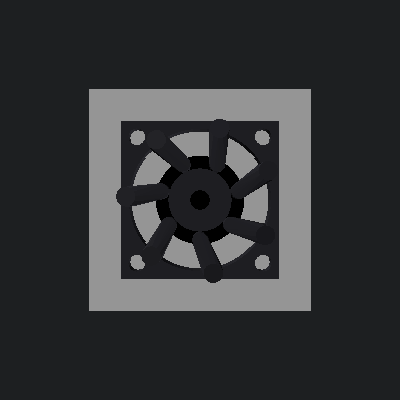
\includegraphics[width=1.5cm,height=1.5cm,keepaspectratio]{figures/png/nema_fan/nema_fan_front.png} &
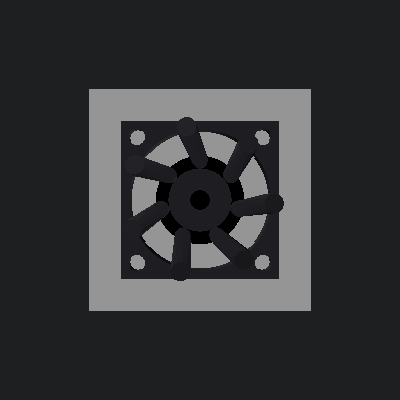
\includegraphics[width=1.5cm,height=1.5cm,keepaspectratio]{figures/png/nema_fan/nema_fan_back.png} &
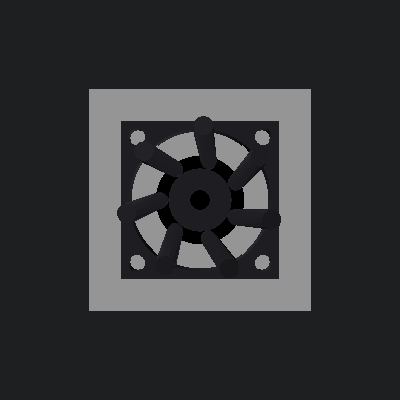
\includegraphics[width=1.5cm,height=1.5cm,keepaspectratio]{figures/png/nema_fan/nema_fan_left.png} &
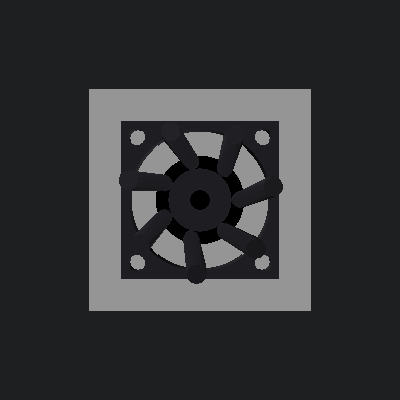
\includegraphics[width=1.5cm,height=1.5cm,keepaspectratio]{figures/png/nema_fan/nema_fan_right.png} &
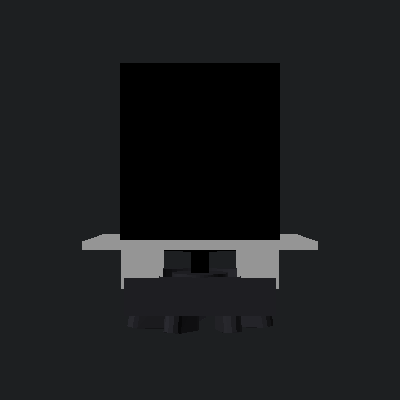
\includegraphics[width=1.5cm,height=1.5cm,keepaspectratio]{figures/png/nema_fan/nema_fan_top.png} &
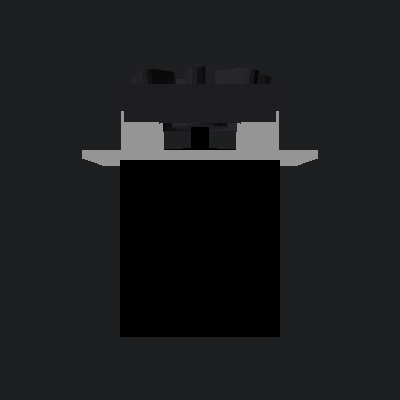
\includegraphics[width=1.5cm,height=1.5cm,keepaspectratio]{figures/png/nema_fan/nema_fan_bottom.png} \\[3pt]

% Row 1.b:3D model of a DC motor with essential structural and functional components
\raggedright 3D model of a DC motor with essential structural and functional components &
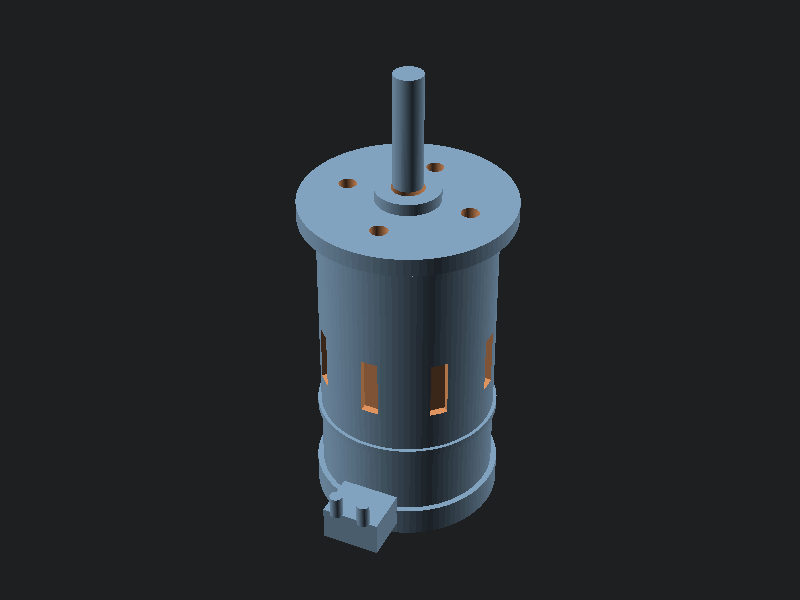
\includegraphics[width=1.9cm,height=1.9cm,keepaspectratio]{figures/png/Dc_motor/Dc_motor_iso.png} &
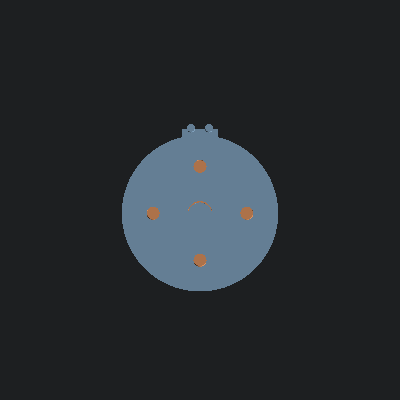
\includegraphics[width=1.5cm,height=1.5cm,keepaspectratio]{figures/png/Dc_motor/Dc_motor_front.png} &

\includegraphics[width=1.5cm,height=1.5cm,keepaspectratio]{figures/png/Dc_motor/Dc_motor_back.png} &
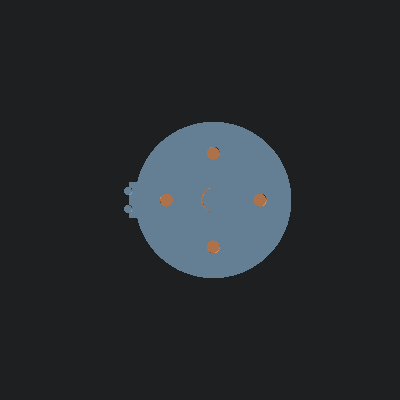
\includegraphics[width=1.5cm,height=1.5cm,keepaspectratio]{figures/png/Dc_motor/Dc_motor_left.png} &
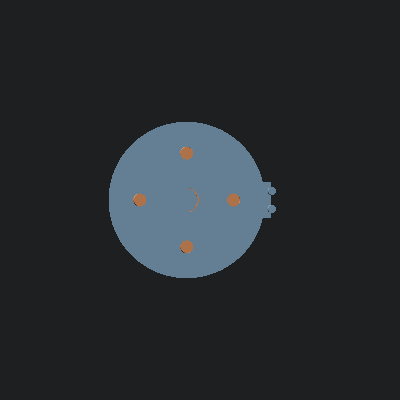
\includegraphics[width=1.5cm,height=1.5cm,keepaspectratio]{figures/png/Dc_motor/Dc_motor_right.png} &
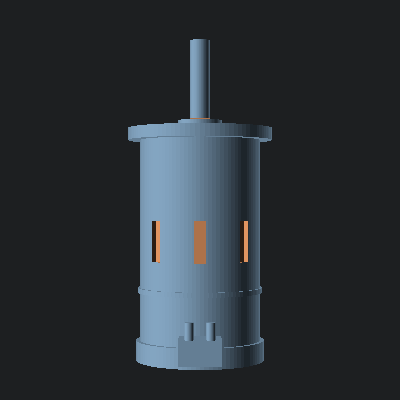
\includegraphics[width=1.5cm,height=1.5cm,keepaspectratio]{figures/png/Dc_motor/Dc_motor_top.png} &
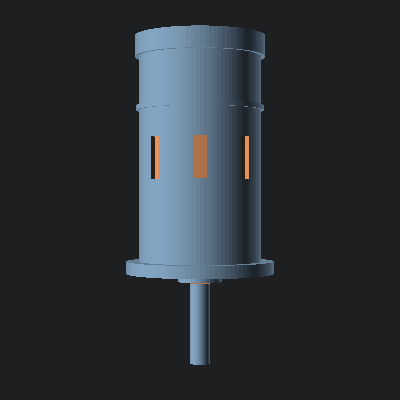
\includegraphics[width=1.5cm,height=1.5cm,keepaspectratio]{figures/png/Dc_motor/Dc_motor_bottom.png} \\[3pt]

% % Row 2: Enclosure (shows internal features)
% \raggedright Electronics enclosure with ventilation slots and cable cutout &
% \includegraphics[width=1.9cm,height=1.9cm,keepaspectratio]{figures/multiview/enclosure_iso.png} &
% \includegraphics[width=1.5cm,height=1.5cm,keepaspectratio]{figures/multiview/enclosure_front.png} &
% \includegraphics[width=1.5cm,height=1.5cm,keepaspectratio]{figures/multiview/enclosure_back.png} &
% \includegraphics[width=1.5cm,height=1.5cm,keepaspectratio]{figures/multiview/enclosure_left.png} &
% \includegraphics[width=1.5cm,height=1.5cm,keepaspectratio]{figures/multiview/enclosure_right.png} &
% \includegraphics[width=1.5cm,height=1.5cm,keepaspectratio]{figures/multiview/enclosure_top.png} &
% \includegraphics[width=1.5cm,height=1.5cm,keepaspectratio]{figures/multiview/enclosure_bottom.png} \\[3pt]

% Row 3: Belt tensioner (mechanical part)
\raggedright Simplified parametric sedan-like passenger car assembly: chassis/body, cabin/roof, bumpers, hood, trunk, windshields, side windows, doors, 4 wheels, and front/rear axles &

\includegraphics[width=1.9cm,height=1.9cm,keepaspectratio]{figures/png/car/iso.png} &

\includegraphics[width=1.5cm,height=1.5cm,keepaspectratio]{figures/png/car/front.png} &

\includegraphics[width=1.5cm,height=1.5cm,keepaspectratio]{figures/png/car/back.png} &

\includegraphics[width=1.5cm,height=1.5cm,keepaspectratio]{figures/png/car/left.png} &

\includegraphics[width=1.5cm,height=1.5cm,keepaspectratio]{figures/png/car/right.png} &

\includegraphics[width=1.5cm,height=1.5cm,keepaspectratio]{figures/png/car/top.png} &

\includegraphics[width=1.5cm,height=1.5cm,keepaspectratio]{figures/png/car/bottom.png} \\[3pt]


% Row 3:Parametric 40mm axial cooling fan: square frame, central hub/bore, twisted blades, 4 mounting holes, corner rounding, and internal clearance cutouts
\raggedright Parametric 40mm axial cooling fan: square frame, central hub/bore, twisted blades, 4 mounting holes, corner rounding, and internal clearance cutouts &
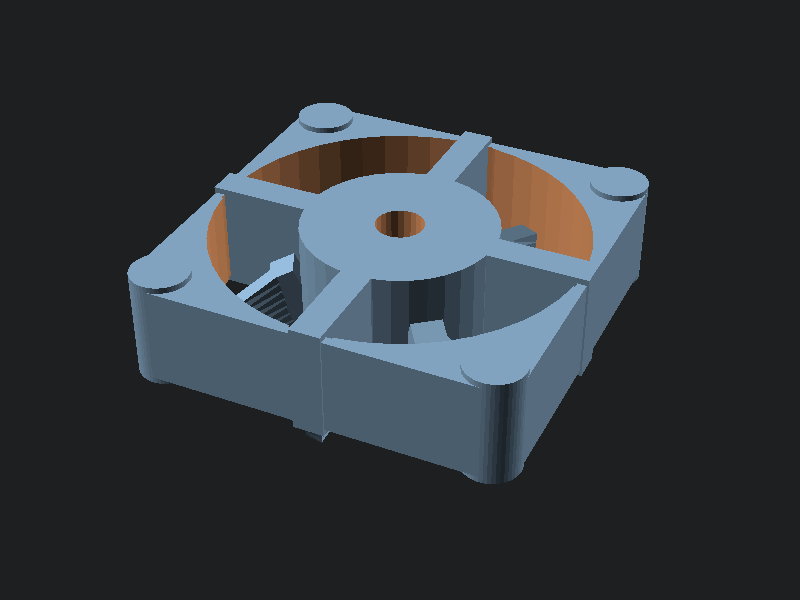
\includegraphics[width=1.9cm,height=1.9cm,keepaspectratio]{figures/png/Cooling_fan/iso.png} &

\includegraphics[width=1.5cm,height=1.5cm,keepaspectratio]{figures/png/Cooling_fan/front.png} &

\includegraphics[width=1.5cm,height=1.5cm,keepaspectratio]{figures/png/Cooling_fan/back.png} &

\includegraphics[width=1.5cm,height=1.5cm,keepaspectratio]{figures/png/Cooling_fan/left.png} &

\includegraphics[width=1.5cm,height=1.5cm,keepaspectratio]{figures/png/Cooling_fan/right.png} &
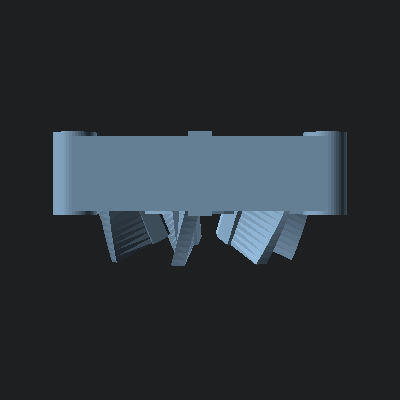
\includegraphics[width=1.5cm,height=1.5cm,keepaspectratio]{figures/png/Cooling_fan/top.png} &
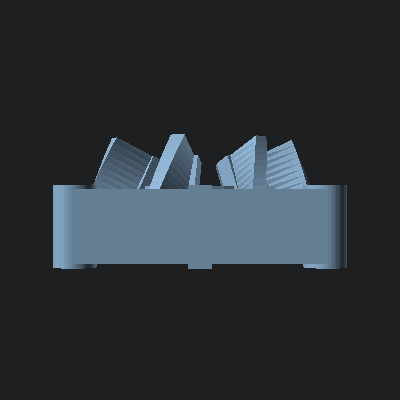
\includegraphics[width=1.5cm,height=1.5cm,keepaspectratio]{figures/png/Cooling_fan/bottom.png}\\[3pt]

% Row 4: Coffee mug (everyday object)
\raggedright Coffee mug with ergonomic handle &
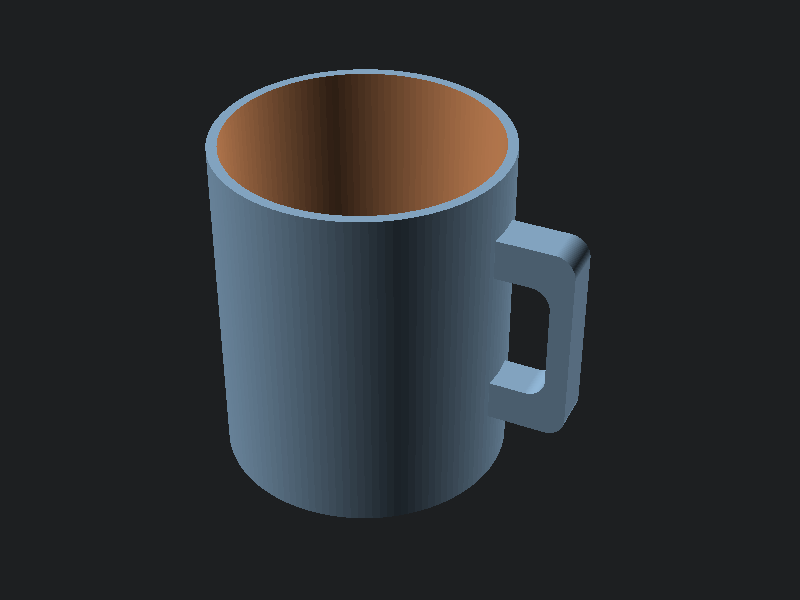
\includegraphics[width=1.9cm,height=1.9cm,keepaspectratio]{figures/png/Coffee_mug/Coffee_mug_iso.png} &
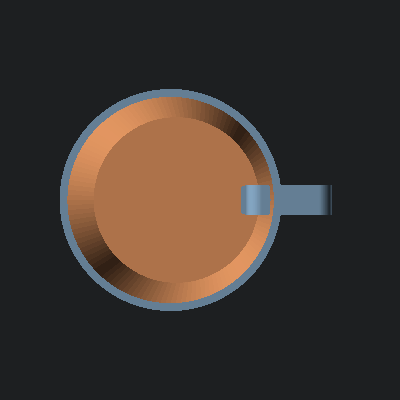
\includegraphics[width=1.5cm,height=1.5cm,keepaspectratio]{figures/png/Coffee_mug/Coffee_mug_front.png} &
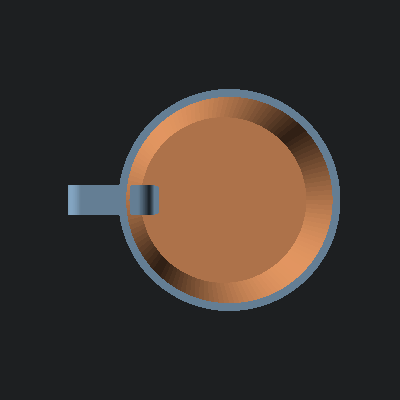
\includegraphics[width=1.5cm,height=1.5cm,keepaspectratio]{figures/png/Coffee_mug/Coffee_mug_back.png} &

\includegraphics[width=1.5cm,height=1.5cm,keepaspectratio]{figures/png/Coffee_mug/Coffee_mug_left.png} &

\includegraphics[width=1.5cm,height=1.5cm,keepaspectratio]{figures/png/Coffee_mug/Coffee_mug_right.png} &
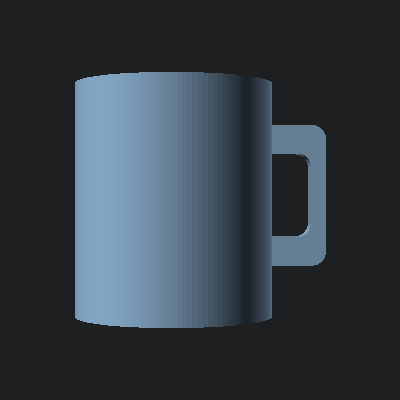
\includegraphics[width=1.5cm,height=1.5cm,keepaspectratio]{figures/png/Coffee_mug/Coffee_mug_top.png} &
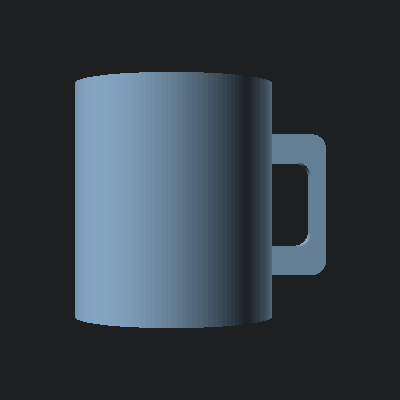
\includegraphics[width=1.5cm,height=1.5cm,keepaspectratio]{figures/png/Coffee_mug/Coffee_mug_bottom.png} \\

\bottomrule
\end{tabular}
\end{figure*}

\begin{table}[t]
\centering
\caption{Geometric and visual similarity across complexity levels. Lower CD indicates closer geometric match; higher F-score, V-IoU, and SSIM indicate better reconstruction. Ground truth models are authored using parametric specifications from NopSCADlib~\cite{nopscadlib}. We evaluate 15 prompts (5 per level). Failed renders are penalized (F-score=0, V-IoU=0, SSIM=0; CD set to $1.5\times$ the observed maximum) so all methods are compared over the same $N$ items. For each complexity tier, we report the best CADence configuration (with or without RAG).}
\label{tab:complexity-comparison}
\setlength{\tabcolsep}{3pt}
\begin{tabular}{llcccc}
\toprule
\textbf{Complexity} & \textbf{Method} & \textbf{CD}$\downarrow$ & \textbf{F}$\uparrow$ & \textbf{V-IoU}$\uparrow$ & \textbf{SSIM}$\uparrow$ \\
\midrule
\multirow{3}{*}{Simple (5)}
  & GPT-4o (direct)      & 6.92  & 0.413 & 0.299 & 0.915 \\
  & GPT-5.2 (direct)     & \textbf{2.28}  & 0.590 & 0.398 & \textbf{0.929} \\
  & CADence + RAG        & 2.55  & \textbf{0.659} & \textbf{0.512} & 0.926 \\
\midrule
\multirow{3}{*}{Medium (5)}
  & GPT-4o (direct)      & 7.57  & 0.196 & 0.108 & 0.887 \\
  & GPT-5.2 (direct)     & 7.03  & 0.232 & 0.076 & \textbf{0.893} \\
  & CADence              & \textbf{5.68}  & \textbf{0.282} & \textbf{0.146} & 0.876 \\
\midrule
\multirow{3}{*}{Complex (5)}
  & GPT-4o (direct)      & \textbf{10.20} & 0.122 & 0.075 & \textbf{0.871} \\
  & GPT-5.2 (direct)     & 12.44 & 0.159 & \textbf{0.125} & 0.687 \\
  & CADence + RAG        & 10.98 & \textbf{0.183} & 0.092 & 0.857 \\
\bottomrule
\end{tabular}
\end{table}

Table~\ref{tab:complexity-comparison} reports geometric and visual similarity between generated models and NopSCADlib-dimensioned reference models across three complexity levels. Since the ground truth is authored using parametric specifications from the NopSCADlib catalog---with exact bearing diameters, mounting hole patterns, and housing dimensions---the reference geometry is dimensionally accurate and independently verifiable against published component datasheets. Failed renders are penalized (F-score, V-IoU, and SSIM set to 0; CD set to $1.5\times$ the observed maximum) so that all methods are compared over the same number of items. For each tier, we report the best CADence configuration (with or without RAG). For simple prompts (basic components such as bearings, washers, and pulleys), GPT-5.2 achieves the lowest CD (2.28) while CADence + RAG leads on surface overlap (F-score 0.659) and volumetric agreement (V-IoU 0.512). The structured pipeline does not provide a meaningful CD advantage for components with basic geometry, but its multi-stage refinement already improves surface and volumetric fidelity.

The benefit of the multi-stage pipeline becomes apparent at medium complexity. Here, designs feature multiple interacting geometric elements---mounting holes, bearing pockets, shaft bores, flanges---where maintaining correct spatial relationships is critical. CADence achieves the best result across three of the four metrics at this level (CD 5.68, F-score 0.282, V-IoU 0.146), as retrieval of standard component specifications (e.g., NEMA~17 mounting dimensions, 608 bearing tolerances) provides domain knowledge that direct generation must infer from parametric knowledge alone.

At high complexity, designs such as multi-part assemblies (belt tensioners, shaft couplers), enclosures (Raspberry Pi~4 case, ESP32 project box), and precision components (T8 leadscrew nut block) present significant geometric challenges. The reference models include detailed port cutouts, bearing pockets, and mounting patterns derived from NopSCADlib specifications. GPT-4o achieves the best CD (10.20) and SSIM (0.871) at this level, aided by its 100\% render rate---GPT-5.2's single failure incurs a steep penalty (CD 12.44, SSIM 0.687). CADence + RAG leads on F-score (0.183), while GPT-5.2 retains the best V-IoU (0.125) thanks to a strong shaft-coupler result. The observation that RAG helps more at medium complexity while the pipeline's iterative refinement drives surface-accuracy gains at high complexity suggests complementary strengths of knowledge retrieval and visual self-correction.


\subsection{Qualitative Examples}

Figure~\ref{fig:comparison} shows representative generations across complexity levels. Direct LLM generation succeeds on simple primitives but degrades on functional objects and multi-part assemblies. CADence maintains structural coherence through its JSON intermediate representation and multi-view VLM feedback. For mechanical components, the RAG system retrieves accurate specifications from NopSCADlib, producing designs with correct mounting patterns and standard dimensions.

Common failure modes include incorrect relative proportions for complex assemblies, missing implicit features not mentioned in prompts, and timeout on designs requiring extensive CSG operations. The error recovery system addresses many but not all of these issues.

Figure~\ref{fig:gallery} presents a broader gallery of representative CADence outputs selected from our evaluation of over 150 diverse prompts. These examples span mechanical components, everyday objects, and abstract geometric designs, illustrating the system's versatility across design categories without any task-specific training.

\begin{figure*}[t]
\centering
\includegraphics[width=\textwidth]{figures/png/cadence_gallery.png}
\caption{Gallery of representative CADence outputs from our evaluation of over 150 diverse text prompts. The designs span a wide range of categories---mechanical components, everyday objects, and abstract geometric forms---demonstrating the breadth of the zero-shot generation pipeline without any task-specific fine-tuning.}
\label{fig:gallery}
\end{figure*}

\subsection{Computational Efficiency}

Average generation time varies substantially with prompt complexity: simple designs complete in approximately 65 seconds, medium-complexity designs in 195 seconds, and complex multi-part assemblies in over 800 seconds (Table~\ref{tab:vlm-ablation} and evaluation logs). The long tail for complex designs reflects additional VLM correction and component verification iterations. VLM assessment accounts for approximately 46\% of total generation time when three correction iterations are used, with the remaining time split between LLM planning/compilation and OpenSCAD rendering. The JSON planning stage itself is fast (under 5 seconds) due to the smaller context required compared to full code generation.

Memory usage remains modest, with peak consumption under 4GB even for complex multi-component designs. The system processes prompts sequentially in our evaluation, but the architecture supports parallelization across the six rendering views and independent component verification.



%% ============================================================
\section{Discussion}
\label{sec:discussion}
%% ============================================================
\subsection{Advantages of Zero-Shot Generation}

The zero-shot paradigm offers several practical advantages. New design categories can be addressed immediately without collecting training data or waiting for fine-tuning. The system benefits automatically from improvements in underlying foundation models. Prompt engineering allows rapid iteration on generation quality without retraining.

However, zero-shot generation has limitations. Fine-tuned models can learn domain-specific conventions and preferences that are difficult to specify in prompts. For high-volume applications in narrow domains, the economics may favor task-specific training despite its upfront costs.

More broadly, CADence represents a paradigm shift in text-to-CAD generation. Concurrent methods follow a \emph{data-scaling paradigm}: collect massive datasets of text-CAD pairs, then fine-tune models to learn the mapping. CADence demonstrates a \emph{knowledge-augmented zero-shot paradigm}: instead of training on hundreds of thousands of synthetic examples, we integrate real engineering knowledge at inference time via retrieval-augmented generation from established component libraries. This distinction has practical consequences---the data-scaling approach requires re-training when new component families emerge, while the knowledge-augmented approach extends to new domains simply by updating the retrieval corpus.

\subsection{The Role of Intermediate Representations}

The JSON IR proves valuable beyond error localization. It serves as documentation of design intent, can be version-controlled alongside generated code, and enables systematic analysis of generation patterns. Future work could exploit this structure for design retrieval, similarity search, and automated refactoring.

The representation also opens paths to multi-backend generation as future work. Because the JSON plan is independent of any target language, it could in principle compile to CadQuery, FreeCAD, or other targets, enabling CADence to serve as a frontend for diverse CAD ecosystems. We have not yet implemented alternative backends, but the architecture supports this extension without changes to the planning stages.

\subsection{Modularity and Model Selection}

The modular architecture of CADence extends beyond error recovery to model selection itself. Each pipeline stage can be independently configured through environment variables, enabling straightforward substitution as newer models become available. Our model configuration comparison (Table~\ref{tab:model-config}) demonstrates that no single configuration dominates across all metrics: GPT-5.2 excels at validation quality (95.2) while the hybrid configuration achieves superior parts detection (98.3\%). This suggests that optimal model allocation may vary by application requirements.

The practical implications are significant. Organizations can balance API costs against output quality by selecting appropriate models for each stage---using faster, cheaper models for deterministic compilation while reserving reasoning models for visual assessment. Researchers can ablate individual components to study their contribution to overall performance. As foundation models continue to improve, CADence can incorporate new capabilities without architectural changes; upgrading from GPT-5.2 to a future GPT-6 requires only configuration updates rather than code modifications. This future-proofing distinguishes CADence from fine-tuned approaches that become obsolete as base models evolve.

\subsection{Limitations}

Several limitations warrant acknowledgment. First, the 6-view assessment, while more comprehensive than single-image approaches, still cannot capture all geometric issues. Internal features, hidden surfaces, and precise dimensional tolerances may escape visual detection.

Second, the system inherits limitations from its underlying models. Complex spatial reasoning remains challenging for current LLMs, and very abstract prompts may receive inconsistent interpretations across runs.

Third, OpenSCAD as a target format, while excellent for parametric modeling, lacks some features of industrial CAD systems. Constraint-based sketching, filleting and chamfering through geometric operations, and assembly constraints are either absent or must be approximated through CSG.

Fourth, evaluation on human-created prompts may not reflect the distribution of real design tasks. User studies with practicing designers would provide stronger evidence of practical utility.

\subsection{Future Directions}

Several extensions merit investigation. Hybrid approaches could combine zero-shot generation with lightweight fine-tuning, preserving flexibility while improving domain-specific performance. Integration of geometric rewards alongside VLM feedback could provide complementary signals for correction. Multi-modal inputs beyond images, such as sketches or existing CAD files, could expand the system's applicability.

The modular architecture facilitates such extensions. Individual components can be replaced or augmented without restructuring the entire pipeline, enabling incremental improvement and experimentation.



%% ============================================================
\section{Conclusion}
\label{sec:conclusion}
%% ============================================================

We presented CADence, a multi-agent pipeline for zero-shot text-to-CAD generation that preserves parametric expressions throughout the generation process. Through a JSON intermediate representation, 6-view VLM assessment, and 5-layer error recovery, CADence achieves competitive results with fine-tuned approaches while offering superior parametric flexibility---without requiring any of the 110K+ training pairs that supervised methods demand.

Our evaluation across over 150 diverse prompts spanning mechanical components, everyday objects, and abstract geometric designs demonstrates the effectiveness of structured generation with comprehensive visual feedback. On a curated geometric benchmark, CADence reduces Chamfer Distance by 45--58\% relative to direct LLM generation on medium and complex designs. Across all evaluations, CADence achieves 100\% compilation and rendering success regardless of model configuration, eliminating the ``no output'' failure mode that limits direct generation approaches. Ablation studies confirm the contribution of each architectural component: VLM self-correction raises approval from 0\% to 66.7\% over three iterations, component verification achieves 86.4\% pass rate on expected parts, and the hybrid model configuration attains 98.3\% parts detection.

CADence demonstrates that the combination of structured intermediate representations, multi-view visual feedback, and progressive error recovery can bridge the gap between zero-shot generation and task-specific fine-tuning for parametric CAD. By producing truly parametric outputs that preserve design relationships, the system enables downstream customization and integration with existing design workflows. We release our implementation to support continued research in this direction.

\section{Declaration of generative AI and AI-assisted technologies in the manuscript preparation process}
During the preparation of this work the author(s) used ChatGPT in order to refine language. After using this tool/service, the author(s) reviewed and edited the content as needed and take(s) full responsibility for the content of the published article.
\clearpage
\section*{References}

\bibliography{references}

\end{document}


